% Created by tikzDevice version 0.12.6 on 2024-07-05 15:51:28
% !TEX encoding = UTF-8 Unicode
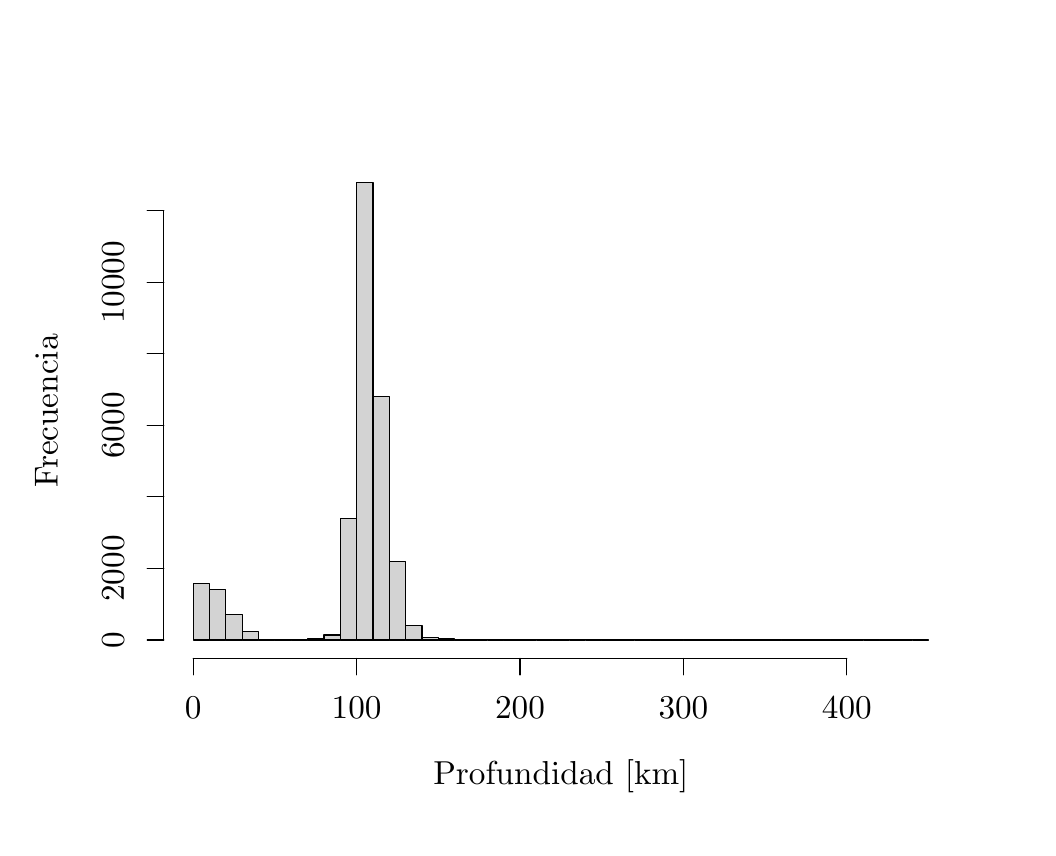
\begin{tikzpicture}[x=1pt,y=1pt]
\definecolor{fillColor}{RGB}{255,255,255}
\path[use as bounding box,fill=fillColor,fill opacity=0.00] (0,0) rectangle (361.35,289.08);
\begin{scope}
\path[clip] (  0.00,  0.00) rectangle (361.35,289.08);
\definecolor{drawColor}{RGB}{0,0,0}

\node[text=drawColor,anchor=base,inner sep=0pt, outer sep=0pt, scale=  1.20] at (192.68, 15.60) {Profundidad [km]};

\node[text=drawColor,rotate= 90.00,anchor=base,inner sep=0pt, outer sep=0pt, scale=  1.20] at ( 10.80,150.54) {Frecuencia};
\end{scope}
\begin{scope}
\path[clip] (  0.00,  0.00) rectangle (361.35,289.08);
\definecolor{drawColor}{RGB}{0,0,0}

\path[draw=drawColor,line width= 0.4pt,line join=round,line cap=round] ( 59.83, 61.20) -- (296.00, 61.20);

\path[draw=drawColor,line width= 0.4pt,line join=round,line cap=round] ( 59.83, 61.20) -- ( 59.83, 55.20);

\path[draw=drawColor,line width= 0.4pt,line join=round,line cap=round] (118.87, 61.20) -- (118.87, 55.20);

\path[draw=drawColor,line width= 0.4pt,line join=round,line cap=round] (177.91, 61.20) -- (177.91, 55.20);

\path[draw=drawColor,line width= 0.4pt,line join=round,line cap=round] (236.96, 61.20) -- (236.96, 55.20);

\path[draw=drawColor,line width= 0.4pt,line join=round,line cap=round] (296.00, 61.20) -- (296.00, 55.20);

\node[text=drawColor,anchor=base,inner sep=0pt, outer sep=0pt, scale=  1.20] at ( 59.83, 39.60) {0};

\node[text=drawColor,anchor=base,inner sep=0pt, outer sep=0pt, scale=  1.20] at (118.87, 39.60) {100};

\node[text=drawColor,anchor=base,inner sep=0pt, outer sep=0pt, scale=  1.20] at (177.91, 39.60) {200};

\node[text=drawColor,anchor=base,inner sep=0pt, outer sep=0pt, scale=  1.20] at (236.96, 39.60) {300};

\node[text=drawColor,anchor=base,inner sep=0pt, outer sep=0pt, scale=  1.20] at (296.00, 39.60) {400};

\path[draw=drawColor,line width= 0.4pt,line join=round,line cap=round] ( 49.20, 67.82) -- ( 49.20,222.89);

\path[draw=drawColor,line width= 0.4pt,line join=round,line cap=round] ( 49.20, 67.82) -- ( 43.20, 67.82);

\path[draw=drawColor,line width= 0.4pt,line join=round,line cap=round] ( 49.20, 93.66) -- ( 43.20, 93.66);

\path[draw=drawColor,line width= 0.4pt,line join=round,line cap=round] ( 49.20,119.51) -- ( 43.20,119.51);

\path[draw=drawColor,line width= 0.4pt,line join=round,line cap=round] ( 49.20,145.35) -- ( 43.20,145.35);

\path[draw=drawColor,line width= 0.4pt,line join=round,line cap=round] ( 49.20,171.20) -- ( 43.20,171.20);

\path[draw=drawColor,line width= 0.4pt,line join=round,line cap=round] ( 49.20,197.04) -- ( 43.20,197.04);

\path[draw=drawColor,line width= 0.4pt,line join=round,line cap=round] ( 49.20,222.89) -- ( 43.20,222.89);

\node[text=drawColor,rotate= 90.00,anchor=base,inner sep=0pt, outer sep=0pt, scale=  1.20] at ( 34.80, 67.82) {0};

\node[text=drawColor,rotate= 90.00,anchor=base,inner sep=0pt, outer sep=0pt, scale=  1.20] at ( 34.80, 93.66) {2000};

\node[text=drawColor,rotate= 90.00,anchor=base,inner sep=0pt, outer sep=0pt, scale=  1.20] at ( 34.80,145.35) {6000};

\node[text=drawColor,rotate= 90.00,anchor=base,inner sep=0pt, outer sep=0pt, scale=  1.20] at ( 34.80,197.04) {10000};
\end{scope}
\begin{scope}
\path[clip] ( 49.20, 61.20) rectangle (336.15,239.88);
\definecolor{drawColor}{RGB}{0,0,0}
\definecolor{fillColor}{RGB}{211,211,211}

\path[draw=drawColor,line width= 0.4pt,line join=round,line cap=round,fill=fillColor] ( 59.83, 67.82) rectangle ( 65.73, 88.31);

\path[draw=drawColor,line width= 0.4pt,line join=round,line cap=round,fill=fillColor] ( 65.73, 67.82) rectangle ( 71.64, 86.19);

\path[draw=drawColor,line width= 0.4pt,line join=round,line cap=round,fill=fillColor] ( 71.64, 67.82) rectangle ( 77.54, 77.07);

\path[draw=drawColor,line width= 0.4pt,line join=round,line cap=round,fill=fillColor] ( 77.54, 67.82) rectangle ( 83.45, 70.88);

\path[draw=drawColor,line width= 0.4pt,line join=round,line cap=round,fill=fillColor] ( 83.45, 67.82) rectangle ( 89.35, 68.06);

\path[draw=drawColor,line width= 0.4pt,line join=round,line cap=round,fill=fillColor] ( 89.35, 67.82) rectangle ( 95.25, 67.95);

\path[draw=drawColor,line width= 0.4pt,line join=round,line cap=round,fill=fillColor] ( 95.25, 67.82) rectangle (101.16, 68.01);

\path[draw=drawColor,line width= 0.4pt,line join=round,line cap=round,fill=fillColor] (101.16, 67.82) rectangle (107.06, 68.18);

\path[draw=drawColor,line width= 0.4pt,line join=round,line cap=round,fill=fillColor] (107.06, 67.82) rectangle (112.97, 69.61);

\path[draw=drawColor,line width= 0.4pt,line join=round,line cap=round,fill=fillColor] (112.97, 67.82) rectangle (118.87,111.60);

\path[draw=drawColor,line width= 0.4pt,line join=round,line cap=round,fill=fillColor] (118.87, 67.82) rectangle (124.78,233.26);

\path[draw=drawColor,line width= 0.4pt,line join=round,line cap=round,fill=fillColor] (124.78, 67.82) rectangle (130.68,155.69);

\path[draw=drawColor,line width= 0.4pt,line join=round,line cap=round,fill=fillColor] (130.68, 67.82) rectangle (136.58, 96.29);

\path[draw=drawColor,line width= 0.4pt,line join=round,line cap=round,fill=fillColor] (136.58, 67.82) rectangle (142.49, 73.00);

\path[draw=drawColor,line width= 0.4pt,line join=round,line cap=round,fill=fillColor] (142.49, 67.82) rectangle (148.39, 68.74);

\path[draw=drawColor,line width= 0.4pt,line join=round,line cap=round,fill=fillColor] (148.39, 67.82) rectangle (154.30, 68.18);

\path[draw=drawColor,line width= 0.4pt,line join=round,line cap=round,fill=fillColor] (154.30, 67.82) rectangle (160.20, 67.96);

\path[draw=drawColor,line width= 0.4pt,line join=round,line cap=round,fill=fillColor] (160.20, 67.82) rectangle (166.11, 67.86);

\path[draw=drawColor,line width= 0.4pt,line join=round,line cap=round,fill=fillColor] (166.11, 67.82) rectangle (172.01, 67.91);

\path[draw=drawColor,line width= 0.4pt,line join=round,line cap=round,fill=fillColor] (172.01, 67.82) rectangle (177.91, 67.87);

\path[draw=drawColor,line width= 0.4pt,line join=round,line cap=round,fill=fillColor] (177.91, 67.82) rectangle (183.82, 67.84);

\path[draw=drawColor,line width= 0.4pt,line join=round,line cap=round,fill=fillColor] (183.82, 67.82) rectangle (189.72, 67.86);

\path[draw=drawColor,line width= 0.4pt,line join=round,line cap=round,fill=fillColor] (189.72, 67.82) rectangle (195.63, 67.84);

\path[draw=drawColor,line width= 0.4pt,line join=round,line cap=round,fill=fillColor] (195.63, 67.82) rectangle (201.53, 67.87);

\path[draw=drawColor,line width= 0.4pt,line join=round,line cap=round,fill=fillColor] (201.53, 67.82) rectangle (207.44, 67.84);

\path[draw=drawColor,line width= 0.4pt,line join=round,line cap=round,fill=fillColor] (207.44, 67.82) rectangle (213.34, 67.84);

\path[draw=drawColor,line width= 0.4pt,line join=round,line cap=round,fill=fillColor] (213.34, 67.82) rectangle (219.24, 67.82);

\path[draw=drawColor,line width= 0.4pt,line join=round,line cap=round,fill=fillColor] (219.24, 67.82) rectangle (225.15, 67.84);

\path[draw=drawColor,line width= 0.4pt,line join=round,line cap=round,fill=fillColor] (225.15, 67.82) rectangle (231.05, 67.84);

\path[draw=drawColor,line width= 0.4pt,line join=round,line cap=round,fill=fillColor] (231.05, 67.82) rectangle (236.96, 67.82);

\path[draw=drawColor,line width= 0.4pt,line join=round,line cap=round,fill=fillColor] (236.96, 67.82) rectangle (242.86, 67.82);

\path[draw=drawColor,line width= 0.4pt,line join=round,line cap=round,fill=fillColor] (242.86, 67.82) rectangle (248.77, 67.83);

\path[draw=drawColor,line width= 0.4pt,line join=round,line cap=round,fill=fillColor] (248.77, 67.82) rectangle (254.67, 67.82);

\path[draw=drawColor,line width= 0.4pt,line join=round,line cap=round,fill=fillColor] (254.67, 67.82) rectangle (260.57, 67.82);

\path[draw=drawColor,line width= 0.4pt,line join=round,line cap=round,fill=fillColor] (260.57, 67.82) rectangle (266.48, 67.82);

\path[draw=drawColor,line width= 0.4pt,line join=round,line cap=round,fill=fillColor] (266.48, 67.82) rectangle (272.38, 67.82);

\path[draw=drawColor,line width= 0.4pt,line join=round,line cap=round,fill=fillColor] (272.38, 67.82) rectangle (278.29, 67.82);

\path[draw=drawColor,line width= 0.4pt,line join=round,line cap=round,fill=fillColor] (278.29, 67.82) rectangle (284.19, 67.82);

\path[draw=drawColor,line width= 0.4pt,line join=round,line cap=round,fill=fillColor] (284.19, 67.82) rectangle (290.10, 67.82);

\path[draw=drawColor,line width= 0.4pt,line join=round,line cap=round,fill=fillColor] (290.10, 67.82) rectangle (296.00, 67.82);

\path[draw=drawColor,line width= 0.4pt,line join=round,line cap=round,fill=fillColor] (296.00, 67.82) rectangle (301.90, 67.86);

\path[draw=drawColor,line width= 0.4pt,line join=round,line cap=round,fill=fillColor] (301.90, 67.82) rectangle (307.81, 67.83);

\path[draw=drawColor,line width= 0.4pt,line join=round,line cap=round,fill=fillColor] (307.81, 67.82) rectangle (313.71, 67.82);

\path[draw=drawColor,line width= 0.4pt,line join=round,line cap=round,fill=fillColor] (313.71, 67.82) rectangle (319.62, 67.83);

\path[draw=drawColor,line width= 0.4pt,line join=round,line cap=round,fill=fillColor] (319.62, 67.82) rectangle (325.52, 67.83);
\end{scope}
\end{tikzpicture}
